\documentclass[12pt]{article}

\usepackage{fullpage}
\usepackage{multicol,multirow}
\usepackage{tabularx}
\usepackage{listings}
\usepackage{pgfplots}
\usepackage[utf8]{inputenc}
\usepackage[russian]{babel}
\usepackage[T2A]{fontenc}
\usepackage{pgfplots}
\usepackage{tikz}


\begin{document}

% \newpage
% \begin{center}
% {\bfseries ФЕДЕРАЛЬНОЕ ГОСУДАРСТВЕННОЕ БЮДЖЕТНОЕ ОБРАЗОВАТЕЛЬНОЕ\\
% УЧРЕЖДЕНИЕ ВЫСШЕГО ОБРАЗОВАНИЯ\\
% «МОСКОВСКИЙ АВИАЦИОННЫЙ ИНСТИТУТ\\
% (НАЦИОНАЛЬНЫЙ ИССЛЕДОВАТЕЛЬСКИЙ УНИВЕРСИТЕТ)»}
% \vspace{1cm}

% Журнал лабораторных работ
% \vspace{6em}

% \vspace{\fill}

% \begin{center}
% Москва 2024
% \newpage
% \end{center}

\section*{Лабораторная работа №3\, по курсу компьютерной графики}

\textbf{Тема:} Камера и базовые 3D-трансформации\\
\\
\textbf{Задача:} Научиться работать с камерой в 3D-пространстве, управлять её положением и направлением, а также освоите базовые трансформации объектов в 3D.\\
\textbf{Вариант:} 2.\\
Постройте несколько простых 3D-объектов (кубы, пирамиды, сферы).\\
Реализауйте камеру, которой можно свободно управлять в 3D-пространстве.
Управление камерой должно осуществляться с помощью клавиатуры и мыши.
Дополнительно: Реализуйте "режим полёта", когда камера может двигаться свободно в любом направлении.

\subsection*{1 Решение}
Для выполнения данной лабораторной работы я использовал OpenGL, так как эта библиотека хорошо подходит для работы с 3D-графикой. 
Основной задачей было создать 3D-объекты (кубы, пирамиды, сферы) и реализовать управление камерой в 3D-пространстве.
Я начал с построения простых объектов, таких как кубы, сферы и пирамиды, используя базовые функции OpenGL для задания вершин и цветов. 
Для управления камерой в 3D-пространстве я реализовал функции, которые позволяют изменять её позицию и направление с помощью клавиатуры и мыши. 
Также я добавил "режим полёта", который позволяет свободно перемещать камеру в любом направлении.
В конце я вывел все параметры объектов на самый верх кода, чтобы было удобно менять параметры сцены.
Все трансформации, такие как перемещения, вращения и масштабирования объектов, были выполнены с использованием матриц преобразований OpenGL.\\


\begin{figure}[h]

\centering
        
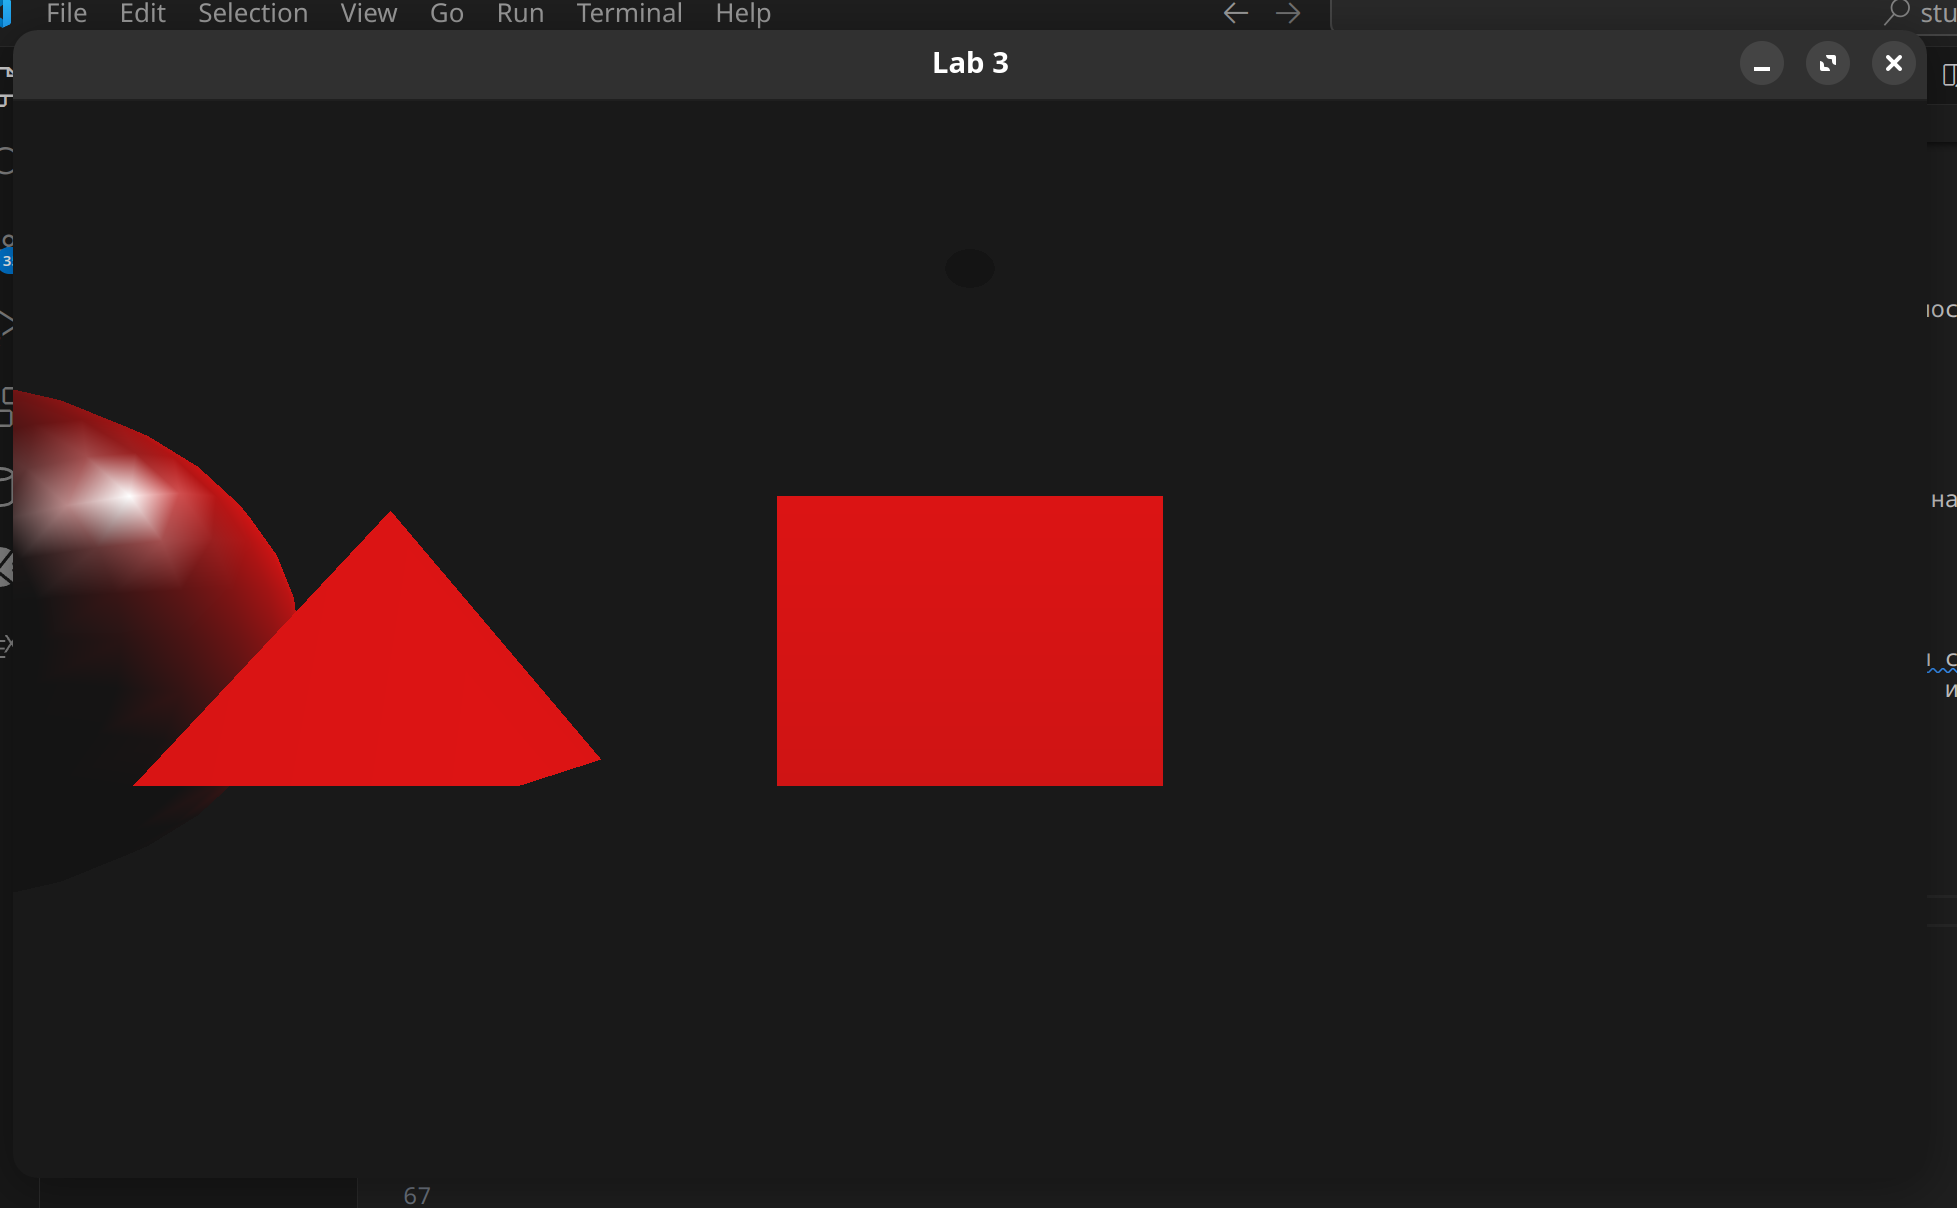
\includegraphics[width=1.0\linewidth]{image.png}
        
\caption{Пример работы программы}
        
\label{fig:mpr}
        
\end{figure}

\subsection*{2 Вывод}
В ходе лабораторной работы была реализована камера, управляемая с помощью клавиатуры и мыши, с возможностью свободного перемещения в 3D-пространстве ("режим полёта"). 
Были созданы простые 3D-объекты (кубы, пирамиды, сферы) с возможностью трансформации (перемещения, масштабирования). Также была настроена чувствительность мыши для удобного управления.
Работа помогла освоить основы работы с камерой и базовыми 3D-трансформациями в OpenGL, а также улучшить навыки управления объектами в 3D-пространстве.



\end{document}
